\section{Background} \label{sec:method}

	\subsection{Ancillary Services} % (fold)
	\label{sub:ancillary}
	Ancillary services are acquired by TSOs in order to ensure the stability of the system and they can generally be divided into primary, secondary and tertiary ancillary services \cite{Rebours}. Each class of ancillary services has a different purpose in grid operation and works on different time scales.

	In the Danish system, producers, represented by a Balance Responsible Party (BRP), are allowed to bid into the ancillary-services market once they have been approved by the TSO. In order to be approved, the producers must prove that they are able to deliver the relevant services within the requirements defined in \cite{EnerginetAncillary,bondy2013}. Here, the TSO defines the bounds of error in service delivery, e.g. how much deviation with respect to a reference power schedule can be accepted before the service is considered non-delivered. In this work, the QoS measures the deviations from the contracted behavior.

	Furthermore, it is expected that new ancillary services will appear in the near future \cite{ipower2013development}. The two main problems that the DSO seeks to solve are congestion issues, i.e. overloading of cables or transformers, and voltage issues. Throughout this paper, the recurring example of an ancillary service is the \emph{PowerMax}, one of the new DSO services. This service is discussed further in Sec.\ref{sub:example}.
	% subsection ancillary_services (end)
	
	\subsection{Asset Management Service} % (fold)
	\label{sub:asset}
	Since the flexibility of individual DERs is too small to provide services to the system operators, an Aggregator pools the flexibility of the units, and presents their flexibility in the market as a single entity, see Fig.\ref{fig:systemarch}. Thus, the Aggregator is responsible for managing the DER units according to certain requirements defined by the owners, hereby providing an asset management service. This service must respect the primary function of the DER. 
	
	By changing the consumption behavior of DER units, the Aggregator performs Demand Side Management (DSM), providing ancillary services to the DSO or, through a BRP, the TSO. The Aggregator and the BRP could be the same entity, but if they are not, the Aggregator should not work against the balancing responsibilities of the BRP.  
	
	\begin{figure}[t]  % Find out how to send it to next column.
		\centering
		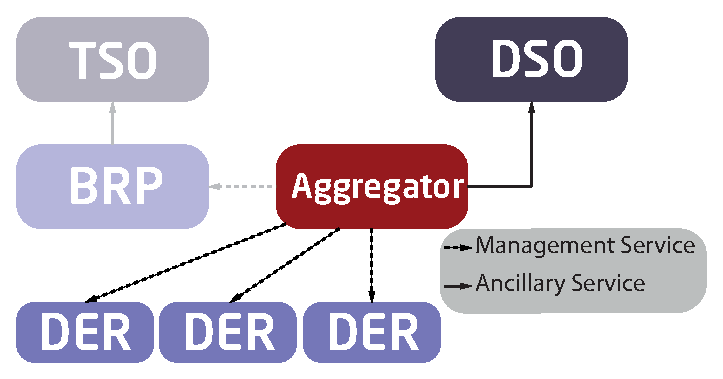
\includegraphics[width=0.7\textwidth]{isgt2014/system.eps}
		\caption{The setup of the power system with DSM. Note that the Aggregator can either be an independent entity or can be a role inside a BRP.}\label{fig:systemarch}
	\end{figure}
	
%	The objective of a DER is to satisfy the needs of its owner. The Aggregator provides the DER owners with an asset management service that ensures the QoS to customers is adequate. Providing services to the grid is only a secondary (and optional) function of the DER, which the Aggregator must take advantage of within the constraints of the primary function. 
	
%	The power consumption of DERs varies greatly depending on the daily routines of their owners and the meteorological conditions. Due to the varying load size, behavior and distributed nature of the DERs, the Aggregator must be able to evaluate if its control algorithms are capable of providing ancillary services and asset management satisfactorily.

	% subsection asset_management_service (end)
	
	\subsection{Control Performance Assessment}
	There is a field of theory on evaluation of controllers: Control Performance Assessment (CPA). Applications of this theory are found mostly in the process industry; for a thorough overview of its applications we refer to \cite{jelali2006overview,Green}. 

		Typically, CPA methods fall within two approaches. One approach, first introduced in \cite{Harris1989}, is to benchmark controller performance against a theoretical optimum, while taking the stochasticity of the system into account. The second approach is to benchmark against deterministic properties the closed-loop system must have, e.g. settling time and steady-state error \cite{Astrom}. In both cases, the index is usually scaled such that:
\begin{equation}
	\zeta = \frac{J_{opt}}{J_{act}},\label{eq:astrom}
\end{equation}
where $J_{opt}$ is the theoretical optimal (minimum) value of the performance criterion \emph{J} (which is usually impossible to achieve in reality), and $J_{act}$ is the actual measured value of the criterion. Since $J_{opt}<J_{act}$, then $\zeta \in [0,1]$. 
		%Given that the requirements of service delivery are easily translated into time-domain deterministic measures, this work presents a deterministic approach. Using the concepts presented in this section, the performance index is defined in the next section.
%In the following, we propose the application of CPA concepts to DSM.

		According to \cite{Green}, performance criteria used to evaluate a controller usually fall within three categories: Quality, Reliability, and Energy. Quality and reliability are concepts that can be directly related to ancillary service provision. The interpretation of energy-related criteria may be suitable for asset-management purposes but is considered out of scope in this work.% The quality of the control performance is measured by the QoS it provides, both towards the system operators and towards its customers. Reliability is measured as how many times the controller provides a QoS outside the specified limits.
